\documentclass[a4paper,10pt,epsfig,epsf,amsfonts,amsmath]{article}
\usepackage[utf8]{inputenc}
\usepackage{ifxetex}
\ifxetex
\usepackage{fontspec}
\setmainfont{TeX Gyre Pagella}
\else
  \pdfoutput=1
  \usepackage[utf8]{inputenc}
\usepackage{textcomp}
\renewcommand{\rmdefault}{phv}
\renewcommand{\sfdefault}{pag}
\renewcommand{\ttdefault}{pcr}
\fi
\usepackage[utf8]{inputenc} 
\usepackage[utf8]{inputenc}
\usepackage[bottom=2cm,top=2cm,left=2.5cm,right=2.0cm]{geometry}

\usepackage{titlesec}

\setcounter{secnumdepth}{4}

\titleformat{\paragraph}
{\normalfont\normalsize\bfseries}{\theparagraph}{1em}{}
\titlespacing*{\paragraph}
{0pt}{3.25ex plus 1ex minus .2ex}{1.5ex plus .2ex}

\providecommand{\xlink}[1]
  {\href{http://arxiv.org/abs/#1}{arXiv:#1}}
\providecommand{\doilink}[2]
  {\href{http://dx.doi.org/#1}{#2}}  
%\textwidth 164mm
\textheight 214mm
%\textheight 247mm
\usepackage{amsmath}
\usepackage{amsthm}
\usepackage{amsfonts}
\usepackage{mathtools}
%\usepackage{color}
\usepackage{graphicx,amssymb,amsmath,dsfont,slashed}

\usepackage[]{units}
%\usepackage[usenames,dvipsnames]{color} % p usar nomes de cores
\usepackage{hyperref}
\usepackage{cite}

\usepackage[usenames,dvipsnames,svgnames,table]{xcolor}
 \definecolor{plum}{rgb}{0.866667,0.627451,0.866667}
\hypersetup{
%   pagebackref,   % page back ref of \bibitem
%     backref=true,	% refs from \bibitem to text
   colorlinks=true,       % false: boxed links; true: colored links
    linkcolor=blue,          % color of internal links
    citecolor=plum,        % color of links to bibliography
    filecolor=magenta,      % color of file links
    urlcolor=YellowOrange           % color of external links
}

%\usepackage{graphicx}
%\input defes.tex
%\documentstyle[12pt,epsfig,epsf,amsfonts,amsmath]{report}
%\makeindex
%\includeonly{}



\usepackage{comment}
\includecomment{instructions}
\specialcomment{instructions}
{\begingroup\itshape }{ \medskip \endgroup}
\excludecomment{instructions}

\includecomment{fapesp}
\specialcomment{fapesp}
{\begingroup\itshape }{ \medskip \endgroup}
\excludecomment{fapesp}

\includecomment{udea}
\specialcomment{udea}
{\begingroup\itshape }{ \medskip \endgroup}
\excludecomment{udea}

\includecomment{instrucciones}
\specialcomment{instrucciones}
{\begingroup\itshape }{ \medskip \endgroup}
\excludecomment{instrucciones}

\includecomment{codi}
\specialcomment{codi}
{\begingroup\itshape }{ \medskip \endgroup}
\excludecomment{codi}

\includecomment{colciencias}
\specialcomment{colciencias}
{\begingroup\itshape }{ \medskip \endgroup}
\excludecomment{colciencias}

\includecomment{evaluacioncodi}
\specialcomment{evaluacioncodi}
{\begingroup\itshape }{ \medskip \endgroup}
\excludecomment{evaluacioncodi}


\includecomment{ideas}
\specialcomment{ideas}
{\begingroup}{ \medskip \endgroup}
\excludecomment{ideas}

\includecomment{evaluacion}
\specialcomment{evaluacion}
{\begingroup}{ \medskip \endgroup}
\excludecomment{evaluacion}



\includecomment{proyecto}
\specialcomment{proyecto}
{\begingroup}{\endgroup}
%\excludecomment{proyecto}

\includecomment{soloproyecto}
\specialcomment{soloproyecto}
{\begingroup}{\endgroup}
\excludecomment{soloproyecto}

\includecomment{soloficha}
\specialcomment{soloficha}
{\begingroup}{\endgroup}
%\excludecomment{soloficha}


\includecomment{evaluador}
\specialcomment{evaluador}
{\begingroup}{\endgroup}
\excludecomment{evaluador}

\includecomment{ingles}
\specialcomment{ingles}
{\begingroup}{\endgroup}
\excludecomment{ingles}


\includecomment{old}
\specialcomment{old}
{\begingroup}{\endgroup}
\excludecomment{old}



\begin{document}
%
%***************************************************************
%
\thispagestyle{empty}
%\begin{center}
%\parbox{0.03\textwidth}{
%\vspace{-2.7 cm}
%\hspace{-7.7 cm} 
\includegraphics[scale=0.2]{unicamp-logo-red}
%\hspace{0.2 cm} 
\includegraphics[scale=0.15]{Ufabc_logo.png}
%\hspace{5.5 cm} 
\includegraphics[scale=0.08]{1280px-Duke_University_logo.png}
%}
%\parbox{0.03\textwidth}{
%\vspace{2.7 cm}
%\hspace{1.7 cm} \includegraphics[scale=0.2]{logo2-gefan.png}
%}
%\end{center}

\begin{figure}
    \centering
    \begin{minipage}{1.2\textwidth}
        \centering
        
\includegraphics[scale=0.2]{unicamp-logo-red} % first figure
        %\caption{first figure}
%    \end{minipage}\hfill
%    \begin{minipage}{0.5\textwidth}
 %       \centering
        
\includegraphics[scale=0.7]{udea} 
        % second figure
%            \end{minipage}\hfill
%    \begin{minipage}{0.5\textwidth}
%        \centering
        % 
\includegraphics[scale=0.18]{logo-iftunesp} 
    \end{minipage}
    
    
    % \begin{minipage}{0.33\textwidth}
    %     \centering
    %     
\includegraphics[width=0.55\textwidth]{1280px-Duke_University_logo} % third figure
    %     %\caption{second figure}
    % \end{minipage}
\end{figure}

\null
%\vskip 2.cm
%\centerline{\Large \bf  Project}
%\centerline{relacionado ao  Projeto Tem\'atico de Pesquisa}
%\vskip 4.5cm
{\color{blue}
\centerline{ \huge \bf  
 }
 \vskip 0.5cm
 \centerline{ \bf 
 Chamada de Propostas Colaborativas FAPESP – Universidad de Antioquia 2019}
\vskip 1.2cm
\centerline{\huge \bf   Title: Beyond the standard model in neutrino experiments  }
}
\vskip 2cm
\[
\begin{array}{c}
 \mbox{\large Principal Investigators:} \\
\mbox{\large Dr. Orlando L. G. Peres$^\dagger$ and Dr. Diego Restrepo$^*$}\\
\\
\mbox{\large Associated Researchers: }\\
\mbox{\large %Dr. Marcelo Moraes Guzzo$^{\dagger}$, Dr. Ernesto Kemp$^{\dagger}$,
Dr. Ettore Segreto$^\dagger$ Dr. Jaime Osorio$^*$, Dr. \'Oscar Zapata$^*$,  Dr. Fabian Casta\~no$^*$}\\
\mbox{\large Master Students: }\\
\mbox{\large 
NN$^*$
}
\\
\\
\mbox{\Large $^\dagger$ Instituto de F\'\i sica Gleb Wataghin - UNICAMP}\\
\mbox{\Large * Universidad de Antioquia (UDEA)} \\
\\
\\
\\
\mbox{\large {\color{magenta}2022 -- 2024}}
\end{array}
\]
\vfill

\newpage

\begin{fapesp}
  See:  http://www.fapesp.br/en/13034
  
FAPESP considers eligible to submit proposals to this call:
  
3.1. Principal Investigators of ongoing research projects funded by FAPESP within the following FAPESP funding modalities: Regular Research Awards (excluding mobility projects), Thematic Projects, Young Investigators, Research, Innovation and Dissemination Centers (CEPIDs/RIDCs), Public Education Research Program, Research in Public Policies, and Research Partnership for Technological Innovation (PITE). Co-Principal Investigators of ongoing Thematic Projects, CEPIDs/RIDCs and PITEs are also eligible to apply.

4.2. For the exchange activities within the scope of this Call are eligible the team members of the related ongoing research award described above in item 3, when previously defined in the ongoing research project as:

a. Principal or Co-Principal Investigators;

b. Associated Researchers affiliated to Higher Education and Research Institutions in the State of São Paulo.

(i) Associated Researchers who are Post-doctoral fellows must have an ongoing FAPESP fellowship during the planned exchange mission.

THE CANDIDATES MUST BE FORMALLY DESCRIBED AS MEMBERS OF THE ONGOING RESEARCH PROJECT.
\end{fapesp}

\begin{udea}
  http://www.fapesp.br/12842
  5. Financiación

a) La UdeA asumirá la financiación de sus respectivos equipos de investigación procedentes de Colombia y la FAPESP la de los equipos de investigación del Estado de São Paulo, Brasil, siempre de conformidad con sus normas nacionales y la disponibilidad de presupuesto.
\end{udea}
\begin{instructions}
A Research Project having a maximum of five (5) pages of scientific content, written in English jointly by the Principal Investigator at the Host Institution in the State of São Paulo and the Principal Investigator at the UNIVERSIDAD DE ANTIOQUIA. One copy of the Research Project shall be sent to FAPESP and an identical copy to the UNIVERSIDAD DE ANTIOQUIA.
\end{instructions}
\begin{udea}
  6.2 The following additional documents required by UNIVERSIDAD DE ANTIOQUIA:

6.2.1 In addition to the above referred research project, the proposal for UNIVERSIDAD DE ANTIOQUIA must include the following items:

a. Approval of the Department Head or Dean of the dependency or whoever takes their place;

b. Detailed budget.

6.2.2 Letter of Agreement of the Host Institution in the State of São Paulo to which the PI from São Paulo is affiliated. The same document is required by FAPESP in item 6.2.3 at www.fapesp/sprint/call32019. The Letter of Agreement may be delivered after the notification of results of this call for proposals and before the grant agreement signature.

7. Submission of proposals to UNIVERSIDAD DE ANTIOQUIA

Submissions can only be accepted electronically via email to viceinvestigacion@udea.edu.co with copy to investigacioninter@udea.edu.co.
\end{udea}

\newpage

 
{\bf ABSTRACT}\\
This is a proposal to search for beyond the standard model signals in neutrino experiments, 
%improve this phrase
associated to non-standard neutrino interactions (NSI).
Based in a recent proposal to parameterize the NSI in terms of Wilson coefficients of effective field theories, 
we want to check the predictions of specific BSM models in this kind of experiments. In particular, we 
will check the change in neutrino production associated to BSM models with new heavy mediators, as well as the possible
production of other light states like the dark photons. 
To reach enough sensitivity, the photon detection system in experiments like DUNE need to be improved, and since the team is already in DUNE, we plane to 
make this changes directly in the joint collaboration.


\vspace{1cm}

{\bf RESUMO}\\


\vspace{1cm}

{\bf RESUMEN}\\

\begin{ideas}
    
{Esta es una propuesta para intercambiar actividades entre UNICAMP, el Instituto de Física Teórica UNESP y la Universidad de Antioquia (UdeA) con el fin de trabajar en modelos del sector oscuro y su relación con las masas de los neutrinos. 
Se harán publicaciones que evalúen el alcance de los detectores de materia oscura y de neutrinos para las partículas de materia oscura ligera y, al mismo tiempo, para las interacciones no estándar de neutrinos (NSI). 
Estos estudios pueden dar luz sobre el potencial pasado por alto de una nueva generación de detectores de neutrinos como DUNE, que pueden probar al mismo tiempo la producción y detección de materia oscura ligera en los detectores cercanos y los efectos de nuevas interacciones de neutrinos que pueden cambiar el perfil de las oscilaciones de neutrinos en el detector lejano de DUNE. 
Cada miembro senior de esta colaboración hará al menos un viaje al otro país. También planeamos un evento de ``Hack Days'' de una semana, donde tendremos un taller de lluvia de ideas entre los miembros senior y los estudiantes graduados en Brasil y en Colombia que involucrará a investigadores  y estudiantes graduados. 
Las actividades de intercambio mejorarán en gran medida la eficiencia de la colaboración y nuestro objetivo de continuar esta colaboración más allá del alcance de este proyecto, con el objetivo de obtener títulos de doble graduación entre las dos universidades brasileñas y la universidad colombiana.
%Enviar comentarios
%Historial
%Guardadas
%Comunidad
}
\end{ideas}

%Preliminary abstract:

%Dark symmetry \url{https://arxiv.org/pdf/hep-ph/0702123.pdf}

%See \url{https://arxiv.org/pdf/1903.10505.pdf}

%\url{https://indico.cern.ch/event/721473/contributions/3034874/attachments/1670431/2679723/CERN_Shoe.pdf}

%See Abelian extension of 331 which may be also a dark symmetry:
%\url{https://arxiv.org/pdf/1909.06386.pdf}
% This is a proposal for exchange activities between UNICAMP, UFABC and
% Duke University to work on studies of supernova neutrino sensitivity
% of the Deep Underground Neutrino Experiment (DUNE).  We will produce
% publications evaluating the sensitivity of DUNE to neutrino absolute
% mass, to the neutrino mass hierarchy, and to non-standard neutrino
% interactions from observation of the burst of neutrinos from a
% core-collapse supernova.  These studies will also serve to help
% optimize DUNE's design.  Each senior member of this collaboration will
% make at least one trip to the other country. We plan also a
% one-week ``Hack Days'' event in Brazil involving senior members and
% graduate students.  The exchange activities will greatly enhance the
% efficiency of collaboration.\\

\vspace{3cm}


\vspace{0.7cm}

% Esta \'{e} uma proposta de atividades de interc\^{a}mbio entre a UNICAMP, UFABC e
% Duke University para trabalhar em estudos da sensibilidade aos neutrinos de supernova
% do Deep Underground Neutrino Experiment (DUNE). Iremos produzir
% publica\c{c}\~{o}es avaliando a sensibilidade do DUNE \`{a} massa absoluta dos neutrinos, \`{a} hierarquia de massa, e \`{a}s intera\c{c}\~{o}es n\~{a}o-padr\~{a}o,
% atrav\'{e}s da observa\c{c}\~{a}o da rajada de neutrinos de uma
% supernova de colapso gravitacional. Esses estudos tamb\'{e}m servir\~{a}o para ajudar a
% otimizar o design do DUNE. Cada membro s\^{e}nior desta colabora\c{c}\~{a}o deve
% fazer pelo menos uma viagem para o outro pa\'{i}s. Tamb\'{e}m  planejamos um
% evento de uma se\-ma\-na de ``Hack Days'' no Brasil, envolvendo membros seniores e
% estudantes de p\'{o}s-gradua\c{c}\~{a}o. As atividades de interc\^{a}mbio aumentar\~{a}o consideravelmente a efici\^{e}ncia de colabora\c{c}\~{a}o entre os grupos envolvidos.


\newpage

\section*{Research project}

\section{Science goals}
Probe BSM models in DUNE
% We propose a collaborative research project in the links between dark matter and neutrinos
% between UNICAMP, UNESP and Universidade of  Antioquia.



% This needs to be written at an accessible level for a general audience

% \subsection{Phenomenological problems}


% \subsection{Specific studies }


% We propose to study the observability of these dark sectors in
% neutrino detectors, in additiona to the signals expected directly o
% inderectly in the usual dark matter probes. Morewever we want to
% explore the possibility of complementarity of Dark Matter detectors to
% check the properties of neutrinos, specially for the next generation
% of direct detection of dark matter models that will be start reaching
% the neutrino floor.


% We have already begun a number of these studies in theoretical model
% that explain dark matter and neutrino masses in the context of dark
% sectors~\cite{}. In addition the team have one increasing experience
% in search for the potential of the planned and future neutrino
% detectors.
% % the context of the
% % DUNE Supernova Burst/Low Energy Physics Working Group.  For each
% % topic, about one year of work of 1-2 graduate students supervised by
% % senior personnel is required to complete each publishable study.

\section{Exchange activities}
\begin{instructions}
a.  A substantive description of the exchange activities, emphasizing their relevance. The proposal must state clearly how the exchange activities to be carried out by each team will contribute to the ongoing research project funded by FAPESP and to the research being carried by the Universidad de Antioquia researcher at UNIVERSIDAD DE ANTIOQUIA;

\end{instructions}

We plan several trips of the participants to collaborate on these studies...

% \begin{itemize}
% \item Diego Restrepo will make a trip to Brazil for 15 days during in the second semester of 2020.
% \item Julian Calle  will make a trip to Brazil for 15 days during in the second semester of 2021.  
% \item Oscar Zapata  will make a trip to Brazil for 7 days during in the second semester of 2021.  

%   % for five days week in late 2019 and another for one week in early
% % 2020. The second of these
% % early 2020, will be a ``Supernova Hack Days'' event involving
% % Brazilian collaborators.  Scholberg has previously organized four
% % similar highly successful Hack Days events at Fermilab involving
% % $\sim$10 SNB/LE group members (mostly students) each.  These involve
% % 3-5 days of focused collaborative work.  Holding the event in Brazil
% % will help to get Brazilian collaborators involved.  Two Duke students
% % (Erin Conley and Adryanna Smith) will attend this, and travel funding is
% % included in the budget for them.

% \item XX will make two trips to Brazil during the period,

% \item XX will make two trips to Brazil during the period,  
  
% \item Peres will make one trip to Medellín
%   % of 10 days in late 2019, for
%   % collaborative work.

% \item Pleitez will make one trip to Duke of two weeks in the period between
%   May and August of 2019 for collaborative work. During this visit he will
%   present his work on non-standard interactions at DUNE.

% \item % Zarah will make one trip to Duke of 10 days in late 2019, for
%    % collaborative work.

% \end{itemize}
      
% \section{Schedule}
% \begin{instructions}
%   b. Detailed schedule of the exchange missions to be carried out by the Universidad de Antioquia team at the São Paulo institution and the São Paulo team at the UNIVERSIDAD DE ANTIOQUIA;
% \end{instructions}


% \section{Performance indicators}
% \begin{instructions}
%   c. Performance indicators for the planned activities, indicating the expected results;
% \end{instructions}

% % Progress will be monitored at the regular bi-weekly DUNE SNB/LE
% % Physics Working Group video meetings (held using Zoom), as well as
% % ad-hoc video meetings as needed.  The participants and their students
% % will also report on their work at DUNE collaboration meetings, which
% % are held three times per year.

% We expect \textbf{at least NNN joint publications to result from this
%   collaborative work}: one on
% % the sensitivity of DUNE to neutrino absolute mass,
% one on
% % sensitivity to mass hierarchy, and one on sensitivity to non-standard interactions
% % of neutrinos.


% \section{Candidates' Contributions}
% \begin{instructions}
%   d. A description of each candidate’s contribution to the mission, explaining their expertise to carry out the foreseen activities;
% \end{instructions}

% % Individual other contributions?

% Vicente Pleitez's contributions to the area of physics beyond the standard model can be summarized as follows: Models with 3-3-1 gauge symmetries in particular the so called minimal 3-3-1 model in which the only colorless fermions are the known leptons: electron, muon and lepton tau and their respective active neutrinos i.e., no new leptons are introduced in the model. These leptons belongs to a triplet of $SU(3)$. If new leptons do exist in Nature an interesting possibility is sterile neutrinos. We call these leptons "neutrino" because they carry lepton number in such a way that the $U(1)_L$ symmetry related to the lepton number may be gauged since the introduction of sterile right-handed neutrinos allow the cancellation of the anomalies. Usually it is assumed that $L(\nu_L)=L(\nu_R)=+1$. However, in 2009 we show that another possibility to cancel anomalies are sterile neutrinos with $L=-4$ (two) and $L=+5$. Recently we have used these sort of right-handed neutrinos to implement the scotogenic mechanism to generate active neutrino masses which include also candidates to dark matter.

% Peres is advising 6 PhD students, one Master student and one post-doc and 8 undergraduate students in neutrino phenomenology. One student (Gabriela Stenico) is studying the role of SBND experiment to discover the short-baseline anomalies, the postdoc (Suprabh Prakash) is working on the possibilities to test
% neutrino decay in DUNE experiment and other (Yago Silva) is working on the the expected sensitivity of the JUNO experiment and constraints of the KamLAND experiment due to neutrino decay. Another student (Mariano Chaves) is looking for BSM (Beyond Standard Model) effects when we study neutrino oscillation with wave packets in quantum field theory approach.

% {\color{red} Diego Restrepo  contribuition}

% {\color{red} Julian Calle   contribuition}

% {\color{red}  Oscar Zapata  contribuition}
  
  
%   All of the aforementioned students from Brazilian institutions will directly profit from this collaboration and the visits by XXX and her students.
  
%  All participants included in this proposal will contribute to organization of, and participate
%  directly in,
%  % the ``Hack Days''  in Brazil.

%  \section{Foreseen actions}
%  \begin{instructions}
%    e. Foreseen actions that will add to the impact of the exchange for the UNIVERSIDAD DE ANTIOQUIA and for the Host Institution in the State of São Paulo, e.g. by means of seminars, short courses etc.;
%  \end{instructions}
% %Scholberg will give a seminar and a short course ($\sim$3 lectures) during the first of
% %her visits.  Moura, Kemp and Peres will all give seminars at Duke
% %during their visits.

 
% \section{Plans for future collaborations}
% \begin{instructions}
%   f. Description of how the Principal Investigators in São Paulo and in the UNIVERSIDAD DE ANTIOQUIA intend to prepare a joint research project, resulting from the exchange activities developed from the proposal submitted in this Call, to be submitted to research funding agencies accessible in their regions in order to create a medium-long-term collaboration (up to one page). The applicants must make explicit in the proposal the name of the funding agencies to which the resulting research project will be submitted.
% \end{instructions}
% \begin{udea}
%   g. The UNIVERSIDAD DE ANTIOQUIA might require at the end of the SPRINT evidence that the researchers have submitted a research project to an extramural funding agency.
% \end{udea}

% We expect this collaborative work to continue beyond the end of this
% grant period.
% % Scholberg is currently funded by the Department of
% % Energy Office of High Energy Physics for work on DUNE, and she will
% % include the ongoing collaborative activities with Brazil in future
% % proposals.  From the Brazilian side, the three members are currently
% % funded by a Thematic Project and will include the ongoing activities
% % in new submissions to FAPESP and to federal funding agencies of
% % Brazil.

\section{State of the Art}
\begin{colciencias}
  tiene como finalidad darle sustento teórico al problema planteado y a
la investigación que busca llevarse a cabo, y tiene como objetivo conocer a
profundidad el tema a investigar e identificar los principales avances obtenidos a la
fecha en esa área del conocimiento para orientar la investigación a generar nuevo
conocimiento.
\end{colciencias}
The neutrino experiments are entering in a precision era where the oscillation parameters are
known with high precision. This opens the possibility to measure new physics (NP) related to non-standard interactions (NSI) 
between neutrinos and matter that arise from physics beyond the SM (BSM).

The usual formalism to parameterize the NSI observables in terms of the Quantum Mechanical (QM) treatment of the oscillation process make difficult to relate directly the observables with the underlying BSM physics which would induce them. Because of that, in the last years
%connect with DUNE from the start
with the motivation of the next generation of neutrino experiments like JUNO, HyperKamiokande and DUNE, 
there have been on big effort into reformulate the NSI in terms of Quantum Field Theory (QFT) in such a way that the NSI could be parameterized in terms of Wilson
coefficients of the effective quantum field theory~\cite{}. In this way, the observables of neutrino experiments can be mapped out directly into the Lagrangians of the BSM theories.
For some specific cases it is even possible to map directly the QFT-NSI effective parameters with the corresponding QM-NSI~\cite{1910.02971}. 
%details of the baseline at some point
To achieve this goal (like in the usual production and detection processes at colliders) the full process must be seen as a single QFT process in space and time, including the production, propagation, and the detection of neutrinos or similar light states like sterile neutrinos, axions or dark photons. Under rather general assumptions, this kind of process have been calculated in ~\cite{1910.02971}. The 
differential rate of detected events per target particle is given by
\begin{align}
R_{\alpha \beta}=\frac{N_{S}}{32 \pi L^{2} m_{S} m_{T} E_{\nu}} \sum_{k, l} e^{-i \frac{L \Delta m_{k l}^{2}}{2 E_{\nu}}} \int d \prod_{P^{\prime}} \mathcal{M}_{\alpha k}^{P} \overline{\mathcal{M}}_{\alpha l}^{P} \int d \prod_{D} \mathcal{M}_{\beta k}^{D} \overline{\mathcal{M}}_{\beta l}^{D}\,,
\end{align}
divided in the three parts of the process,
where $d\prod_{P} $ is the phase element for the \emph{production} part,  $\Delta m_{k l}^{2} \equiv m_{k}^{2}-m_{l}^{2}$ is the mass squared difference between neutrino eigenstates in the \emph{propagation} part, $d\prod_{D} $ is the phase element for the \emph{detection} part. The amplitudes $\mathcal{M}_{P,D}$ describe the neutrino production and detection processes. Finally, $N_{S,T}$ are the number of source/target particles separated by a macroscopic distance $L$, $m_{S,T}$ are their masses, and $E_\nu$ is the neutrino energy. In this approach, the
neutrino is an intermediate particle in the amplitude.

%reformulate
non-standard neutrino interactions
\begin{itemize}
    \item Interactions in the production and detection (mostly charged current)
    \item Interactions in the propagation (mostly neutral current)
\end{itemize}



%improve
The information about the specific BSM model is encoded in the corresponding  amplitudes $\mathcal{M}_{P,D}$ which can be calculated from the Lagrangian by using the typical QFT techniques. 
It is convenient to separate each amplitude in two parts: the usual SM interactions
%search 
and the NSI contributions proportional the Wilson coefficients $\epsilon_X$, $X=L,R,S,P,T$ for left, right, scalar, pseudoscalar and tensor interactions respectively. 

\begin{ideas}



From 1910.02971
\begin{quote}
    This opens the door to also probing and constraining new physics (NP), by which we
mean non-standard interactions (NSI) between neutrinos and matter that arise from physics
beyond the SM (BSM) [5–24]. 
\end{quote}
\begin{quote}
    he idea is to treat the neutrino production and detection together as a single process [25]
    [...]    
    In this approach,
neutrino is merely an intermediate particle in the amplitude [...]
The source and the target are separated by a macroscopic distance L.
\end{quote}
\begin{quote}
    We calculate the event rate and oscillation
probability in the presence of general NSI, starting from the effective field theory (EFT) in
which new physics modifies the flavor or Lorentz structure of charged-current interactions
between leptons and quarks. We also provide the matching between the EFT Wilson coefficients and the widely used simplified quantum-mechanical approach, where new physics
is encoded in a set of production and detection NSI parameters.
\end{quote}
\begin{quote}
    describing the number of neutrino
events detected at a distance L from the source, taking into account possible neutrino
oscillations and nonstandard charged-current interactions
\end{quote}
\begin{quote}
    Thus, in this paper we focus on NP in charged-current interactions between neutrino
and matter. The theory framework we consider is the EFT of the SM degrees of freedom at
the energy scale $\mu \approx 2$ GeV, in which lepton-number conserving NP modifies the effective
4-fermion interactions between leptons and quarks
\end{quote}

\begin{quote}
    Eq. (A.21) is quite general. It is valid for any single neutrino production or detection
mechanism, any neutrino interactions, any number of light neutrinos, etc.
\end{quote}

\begin{quote}
    Therefore, neutrino production via pion decays can be described
by the QM-NSI formalism to all orders (with the above matching), even in the presence of
non-SM-like interactions
\end{quote}

\end{ideas}


Standard model effective field theories applied to neutrino phenomenology~\cite{1901.04553,1910.02971,2011.14292}.
Connected directly with~\cite{1901.04553} (\url{https://www.connectedpapers.com/main/61a156d6f312623389f42c0c89fce1b0bf0a700a}) we have also the General neutrino interactions~\cite{1905.08699}, 
connected with the NSI in radiative neutrino mass models~\cite{1907.09498}



%speak about gni
(GNI)

In this project we want to probe BSM theories in neutrino experiments and evaluate the potential of future experiments like DUNE to explore the parameter space of such theories.

For that, we start from the BSM specific Lagrangian and calculate the Wilson coefficients associated to NSI and GNI





\begin{old}
\textit{Dark sectors}: Dark matter (DM) is an important ingredient of
the primordial plasma in the early Universe which left an imprint in
the cosmic microwave background (CMB) with a contribution of the
$27\%$ of the total matter-energy budget of the
Universe~\cite{Aghanim:2018eyx}.
In fact, besides the temperature of the CMB is quite constant along all
directions, the small fluctuations with higher temperatures point out
towards  gravitational potential-wells driven by dark matter.
They are the seeds to capture all the material required for the
formation of the large scale structures of the Universe.
In later stages of the evolution, the DM remains as the main component
of the formed structures. To accommodate the observations related to the excessive
speed of the stars in the external part of the galaxies, and similarly, the
excessive speed of the more external galaxies in galaxy clusters,
the same $27\%$ additional content of the mass-energy budget of Universe
must be in the form of dark matter.

Regarding the DM itself, a piece of evidence about its dark character (very
small interactions with the standard model (SM) photons) comes from
the observation of the Bullet cluster (1E~0657-56).
This cluster is the result of the collision between two clusters with
a relative speed of $\sim 3000~\text{km/s}$ which make it a rare system in the
Universe~\cite{Bouillot:2014hda, Kraljic:2014soa,Thompson:2014zra}.
From the measurements of this system, we can
infer the existence of two DM halos with a very low interaction between
themselves. This has allowed them to have a significant
departure from the region of interaction of the intergalactic gas
identified by the $X$-ray emission of the system.  The reconstruction
of the collision has allowed infering the maximum value of the ratio
of the DM particle self-interactions and its mass in the range
$0.1\lesssim \sigma/m\lesssim 10~\text{cm}^2/\text{g}$~\cite{Spergel:1999mh,
  Wandelt:2000ad, Vogelsberger:2012ku, Rocha:2012jg, Peter:2012jh,
  Zavala:2012us, Vogelsberger:2014pda, Elbert:2014bma,
  Kaplinghat:2015aga}.  However, like what happens with other
gravitational piece of evidences of DM, the possible interaction of the DM
particle with the SM particle content is completely unknown until
now.


Under the hypothesis that the DM is formed by
non-relativistic particles, large scale structure formation
simulations, based on the initial conditions given by the CMB power
spectrum, predict the existence of DM halos containing the galaxies,
and sheets and filaments of DM joining the halos and filled with the
$60\%$ of the primordial gas~\cite{Rodriguez:2018mjb}.
This structure of DM which supports the baryonic content of the
Universe is called the cosmic web.

This view of the Universe is
supported by an overwhelming set of observations related to the
gravitational effects of the DM at all the
scales~\cite{Buckley:2017ijx}.
One of the last pieces of evidence about the existence of this cosmic
web has been recently obtained with the measurement of the gas which
is filling the filament joining two distant galaxy clusters at 
redshift $z\sim 3$~\cite{Umehata2019}.
All this evidence points out to the interpretation
of the dark matter in terms at least of new particle
beyond the standard model.
The full set of gravitational evidence around the dark matter
particle, along with the results from the simulation of large scale
structure formation, allow inferring that the momentum of the DM
particle must be sufficiently low in such way that those particles
cannot be relativistic (hot) but warm or cold after their production
in the early Universe~\cite{Aghanim:2018eyx}.  In this way, the
interpretation of DM as a non-relativist particle is firmly
established.

This has motivated the search and characterization of the particle
responsible for  the DM of the Universe as one of the biggest
experimental efforts today.
There is a vast world program whose goal is to detect the
non-gravitational effects of the dark matter particle, by following
one approach which is multi-channel and multi-messenger.
The main strategies are direct detection, indirect detection
and the production at collider in all the three frontiers in which the
current searches in particle physics are developed: the \emph{energy
  frontier}, the \emph{cosmic frontier}, and the \emph{intensity
  frontier}~\cite{Hewett:2012ns}.  In the energy frontier, one possibility
is the direct production of DM particles in a high luminosity collider,
like the LHC, and the subsequent detection in detectors like
ATLAS~\cite{Tolley:2016lbg} or CMS~\cite{Sirunyan:2016iap}.  The main
signal at LHC corresponds to events with transverse missing energy. In
general, this kind of searches requires large cross-sections for the
particles which are produced along with the DM particles.
The cosmic frontier, on the other hand, make use
of the dark matter already existing in the Universe today in either a
direct way: by using the dark matter around us, or indirectly by
looking at the places where it is expected that densities of dark
matter are larger, like the galactic center or inside dwarf galaxies.
In this frontier, direct detection experiment try to measure the small
recoiling energy of a nucleus of a material stored in a detector after
the collision of a DM particle passing by.  Some of the main
experiments in direct detection of DM are: XENON1T~\cite{Aprile:2018dbl},
LUX~\cite{Akerib:2016vxi}, PandaX-II~\cite{Tan:2016zwf},
LZ~\cite{Mount:2017qzi}, DAMA/LIBRA~\cite{Bernabei:2013xsa}, and
DARWIN~\cite{Aalbers:2016jon}.
The last generation of this kind of experiments is using tons of
material and are pushing the expected limits of DM models with SM
mediators in a wide range of masses.
On the other hand, indirect detection experiments try to measure the
flux of sufficiently stable particles produced by annihilation or
decays of the DM candidate.
Between these particles, the gamma rays are considered as the best
channel for the identification of DM properties, since they preserve
both the spectral and spatial information about the signal.
This is done with detectors installed in satellites like
Fermi-LAT~\cite{Fermi-LAT:2016uux}, and
AMS-02~\cite{Pizzolotto:2016lwk}, or land-based observatories like
H.E.S.S.~\cite{Lefranc:2016srp}, all of which are taking data in the
range expected by the WIMP paradigm.
For the same reasons, neutrinos are considered also a clean channel
that can be detected in huge photomultiplier arrays in
ice, like IceCube~\cite{Aartsen:2016zhm}, or in the sea, like ANTARES~\cite{Albert:2016emp}.
This project will study the potential of the intensity frontier to
explore hidden sectors of dark matter. In experiments of this kind, 
neutrino beams are built for long-baseline experiments along with near
and far detectors. Yet the main goal of them is to measure neutrino
properties, they can be sensitive to the dark sector particles and mediators in models of dark matter related to neutrino physics.

Despite
the plethora of experiments trying to find it, we still do not have direct evidence of
the existence of such a particle or their (self)interactions.
Since the simplest scenarios are quite restricted now, the idea of
having not only one DM particle but a full dark sector sufficiently
hidden from the Standard Model sector, is becoming a very active
research field.

It is expected that observations to smaller scales of the size of
dwarf galaxies, when combined with simulations of structure formation
with baryonic effects, can be sensitive to the properties of the
particles which make the dark matter~\cite{Buckley:2017ijx}.  One
possibility which is emerging from this kind of simulations is that
the dark matter particles have some kind of self-interaction between
them~\cite{Kamada:2016euw, Tulin:2017ara}.  If confirmed, this would
imply big restrictions for the building of models of self-interacting
dark matter (SIDM)~\cite{Bringmann:2016din}.  Shortly it is
expected a substantial improvement in this kind of observations, along
with an increase in computational power to include baryonic effects.
This kind of advances requires that the phenomenological models of dark
matter can calculate more precise predictions. The theoretical program
in this direction must be flexible enough to respond to
(unexpected) dark matter signals and its influence in the
observational programs~\cite{Buckley:2017ijx}.  {\bf In this project} we
have the objective of building theoretical models with features which can
go beyond the WIMP paradigm and may have new implications in this kind
of simulations that include baryonic effects and have the possibility
of be tested by new low scale astronomical observations, especially the
ones in the range of  $10^9$ to  $10^{10}$ solar masses~\cite{Buckley:2017ijx}. 
\end{old}

\begin{ideas}
    
{\bf In this project} we will develop a method to have a very well defined
dark sector related to the problem of neutrino masses to be explained
below.
In this kind of models, the dark photon~\cite{Ren:2018gyx,She:2019skm} is one of the mediators of the
interactions between the dark sector and the standard model and can be
sufficiently light as to generate the kind of self-interactions
expected to have observable effects in the near future structure
formation simulations with baryonic effects.

\textit{Neutrinos} are elementary particles with very tiny masses, and
with almost no interactions with the matter.  Their properties are
connected to a fundamental understanding of particle physics and
cosmology -- the history and evolution of the Universe.
In the past few decades, we have learned an enormous amount
about neutrinos, including that they have tiny but non-zero masses
(the subject of the 2015 Nobel Prize in physics~\cite{premionobel2015a,premionobel2015b}).  Neutrinos come in
six types or ``flavors'', and how neutrino flavors can
change from one to the other tells us about their masses and other a
fundamental properties~\cite{GonzalezGarcia:2002dz}.  In turn, information about neutrino masses
can tell us about the evolution of the Universe, possibly shedding
light on such questions as  why is the Universe made of matter and not
antimatter? How did the structure of the Universe come to be what it
is today?
Within the standard model, neutrino are massless and therefore any
explanation about their tiny masses and mixing require extensions of
the standard model.  The group from UNICAMP have been working on neutrino physics in the last 25 yrs~\footnote{The research in neutrino physics made by the GEFAN group at UNICAMP  is supported by a Thematic Project described in  \href{https://bv.fapesp.br/pt/pesquisador/44012/orlando-luis-goulart-peres/}{https://bv.fapesp.br/pt/pesquisador/44012/orlando-luis-goulart-peres/}.} {\bf In this project we aim to have the predictions of models of particle physics with dark sectors and that at same time have impact on neutrino phenomenologies such as neutrino masses and non-standard neutrino interactions.}

\textit{Simplified models} are minimal standard model extensions which
solve specific phenomenological problems, like the existence of a DM candidate or 
the explanation of tiny neutrino masses.
Current limits, mainly from
the LHC and direct detection, have put severe constraints in simplified
models for Dark Matter with standard model portals. 
In fact, until now, all the searches have reported negative results, without
any signal that can point out unambiguously to the particle 
responsible for the dark matter in the Universe.
Since the evidence of the existence of dark matter as a particle is so strong, 
these negative results are interpreted in the sense that
the models with standard model portals are disfavored by the current experimental limits.
Recently, a good portion of the theoretical effort in this direction
is pointing out towards more complete models which also solve 
other phenomenological problems. 
In general, this requires a wider dark sector which involves
particles with relaxed restrictions from the LHC searches.
Some recent papers along this direction are for
example:~\cite{Restrepo:2019soi,Ghiglieri:2019kbw,Ahmed:2019zxm}.


This has opened the possibility of considering more
\emph{complete models} aimed to explain several phenomenological problems.
{\bf In this project} we aim to build  phenomenological complete
models that can explain both the dark matter and neutrino mass problems.
% which kind of ultraviolet extensions
A good starting point in this direction is the simplified models
based in an Abelian gauge dark symmetry under which the standard model
particles are neutral.  The lightest dark matter particle in the dark
sector can be a good dark matter particle, while the very same
symmetry can forbid three-level contributions to neutrino masses that
can help to explain the smallness in their masses. The enlarged dark
sector required to explain radiative neutrino masses can help to relax
current constraints in dark matter searches through new portals and
co-annihilation processes, while open new and more subtle ways to
search for it.
For example, through the search of dark photons or dark matter related
signals in neutrino detectors~\cite{Bertuzzo:2018itn,Bertuzzo:2018ftf,Arguelles:2019xgp}, the effect of
non-standard interactions emerging from that kind of
models~\cite{Dev:2019anc}, and the impact in cosmological
observables~\cite{Abazajian:2019oqj}.
% How to build them
Recently the first self-consistent renormalizable model along this
line was proposed by the Colombian counterpart of this team~\cite{Calle:2019mxn}.
% What to check
With this project we plan to systematically study this kind of models
with an emphasis in new observables related to neutrino physics, and
in signals of DM particles or DM mediators in present and future
neutrino detectors, and also in DM detectors sensitive to the region
close to neutrino floor.
% Speak about the importance of dark matter detectors in neutrino physics
%\textit{neutrinos themselves}.
The neutrinos are the darkest between the SM particles, in
the sense that they can couple through the neutrino portal $LH$
operator with dark sectors that participate in the generation of
neutrino masses~\cite{Schmaltz:2017oov}.
 

\begin{figure}[hbtp]
\centering
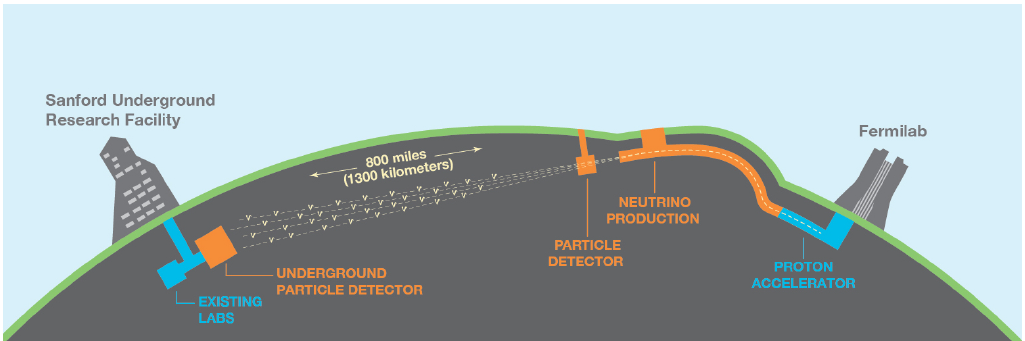
\includegraphics[width=\textwidth]{fig14.png}
\caption{The Deep Underground Neutrino Experiment (DUNE). Schematic diagram of the neutrino beam propagating from Fermilab to Sanford Underground Research Facility (SURF), where the far detector is located.}
\end{figure}

\end{ideas}

%\subsection{The DUNE Experiment}
One of them is
The DUNE experiment (\url{http://dunescience.org}) which has a planned
40-kiloton liquid argon far detector to be installed underground at the
Sanford Underground Research Facility in South Dakota~\cite{Abi:2020evt}.
It is is the flagship particle physics experiment in the U.S., and has
more than 1,000 collaborators from more than 30 countries.  Brazil has
been a collaborating country in DUNE since the collaboration was formed in 2014, and Colombia 
is a recent member of the collaboration with several institutions.

The underground
neutrino detector will be combined with a high-intensity neutrino beam
from Fermilab to study neutrino flavor transition properties.
The near detector is expected to be sensitive to DM signal with low
mass mediators~\cite{Coloma:2015pih}, while the main detector is expected to constraint
a specific region of the parameter space for DM explorations.  Both
detectors are sensitive to dark photon signals~\cite{Bertuzzo:2018itn,Bertuzzo:2018ftf,Arguelles:2019xgp,Bakhti:2018avv,Berryman:2019dme,Machado:2019oxb,Cappiello:2019qsw}.


All the researchers of this project belongs officially to the DUNE collaboration through the two institutions. In particular, UNICAMP plays an important role in the experiment
by leading the Photon Detection System Consortium at DUNE, with the Lepton LAB to produce the Arapuca photon detectors for DUNE, and for leading the efforts of the design the DAPHNE board to received and process the signals from the Photon Detection System. In this project we propose to open new ways to use DAPHNE to characterize components of the photon detection system. 
 In particular, we propose to make studies of the quantum efficiency of the arapucas detectors by taking data with DAPHNE.


% This
% work, however, does not relate to the beam, but rather the potential
% observation of a supernova burst signal.  For that signal, DUNE has
% unique properties: it is sensitive to the \textbf{electron neutrino
%   flavor} of the supernova burst, unlike other detectors.  The
% ``neutronization burst'', a few tens of milliseconds long at the
% outset of the supernova, is the explicit signature of the neutron
% star's birth.


% -----------------------------------------------------------------
% State of the art, electronics of DAPHNE
% -----------------------------------------------------------------
\subsection{DUNE Experiment}

The DUNE (Deep Underground Neutrino Experiment) is an experiment under construction for the study of neutrinos, which was formed in April 2015 and will be fully operational by the year 2027. The Fermilab facilities (in Illinois) will be used for the experiment to produce neutrinos and to install a nearby detector. At 1300 kilometers (Sanford Laboratory in South Dakota) a distant detector will be located (1.5 km below the surface) that will observe the neutrinos produced in Fermilab \cite{Anderson_2012}.

Among the objectives of the DUNE are to investigate the neutrino oscillations to test the violation of CP in the lepton sector, to determine the order of the masses of neutrinos, to study supernovae and the formation of a neutron star or a black hole, to study the decomposition of protons, among others.

In the Sanford Laboratory, at a depth of 1,500 m, 4 tanks (63.6 m long, 16.7 m wide and 15.6 m high) will be built, which will be filled with liquid argon and will serve as detectors for neutrino collisions with atoms of argon. Silicon photon multipliers (SiPM) will be placed around the tanks to record the radiation produced in the collisions of neutrinos with argon atoms. A card called DAPHNE (Electronic Detector to Acquire Photons from Neutrinos) has been developed that will supply the voltage to the silicon photon multipliers (SiPM) and take the data to send them through an optical fiber, each DAPHNE card will control 40 SiPM and register the signal of each SiPM at 65 MHz.


\subsection{Photon Detectors}

\subsubsection{The single-phase Liquid Argon Temporary Projection Chamber (LArTPC)}


The primary physical goals of DUNE are the search for lepton charge parity (CP) violation, the search for nucleon decay as a signature of a Grand Unified Theory underlying the Standard Model, and the observation of neutrino bursts from supernova (SNB) of supernovae. Critical to achieving this physics program is the construction of a detector that combines the multi-kiloton fiducial mass detection needed for rare event searches with subcentimeter spatial resolution in its capability to image those events, allowing us to identify signatures of rare events. The single phase (SP) Liquid Argon Time Projection Chamber (LArTPC) \cite{Rubbia:117852} enables these dual objectives to be achieved by providing a way to read ionization patterns in large volumes of liquid argon (LAr) at subcentimeter granularity, Solar neutrino interactions and SNB to GeV-scale interactions of neutrinos from the Long-Baseline Neutrino Facility (LBNF) beam \cite{Abi_2020_2}.

To search for the lepton violation of CP, the appearance of electron neutrinos $\nu_{e}$ in the LBNF beam of muon neutrinos $\nu_{\mu}$ must be studied. This requires the ability to separate the electromagnetic activity induced by the charged current interactions of $\nu_{e}$ from the similar activity arising from photons. Two signatures allow this: photon showers are usually preceded by a gap before the conversion, characterized by the conversion length of 18 cm in LAr; and the initial part of a photon shower, where an electron-positron pair is produced, has twice the $dE/dx$ of the initial part of an electron-induced drift. It is also vital to accurately identify these nucleon decay events to suppress cosmic muon-induced backgrounds, and here the detection of argon scintillation photons is essential to determine the event's timing.

Detecting an SNB presets different challenges: dealing with a high data rate and maintaining the high detector uptime required to ensure we don't miss one of these rare events. The signature of an SNB is a collection of electron footprints of MeV energy a few centimeters in length distributed throughout the volume of the detector. To completely rebuild an SNB, the entire detector must be read, a data rate of up to 2 TB/s, for 30 s to 100 s, including a pre-trigger window \cite{Abi2017}.

A large volume of LAr is subjected to a strong electric field of a few hundred volts per centimeter. Charged particles passing the detector ionize the argon atoms and the ionization electrons travel in the E-field towards the anode wall on a time scale of milliseconds. This anode consists of layers of active wires that form a grid. The relative voltage between the layers is chosen to ensure that all but the final layers are transparent to drifting electrons, and these first layers produce bipolar induction signals as electrons pass through them.

The final layer collects the drifting electrons, resulting in a monopolar signal. LAr is also an excellent scintillator, emitting UV light at 127 nm. This fast-scintillating light, passing through the detector on a nanosecond time scale, travels into the visible and is collected by photon detector devices (PDs). PDs can provide an initial time determination $t_0$ for events, telling us when the ionizing electrons begin to drift. Relative to this $t_0$, the time at which the ionizing electrons reach the anode allows the reconstruction of the event topology along the drift direction, which is crucial for identifying nucleon decay events and applying drift corrections to ionization charge. The current pattern observed in the grid of the anode wires provides the information for the reconstruction in the two coordinates perpendicular to the drift direction.


\subsection{Photon Detection System}

Compared to ionization electrons, which can take milliseconds to traverse the drift volume, scintillation photons are fast, arriving at DPs within nanoseconds after production. This flashing light provides a t0 for each event. By comparing the arrival time of the ionization at the anode with this t0, reconstruction in the drift direction becomes possible. A 1 µs timing resolution of the PD system allows a position resolution of ∼1 mm for 10 MeV SNB events \cite{Abi_2020_2}.

This must be able to be done throughout the active volume with >99\% efficiency, leading to a requirement of at least 0.5 photoelectrons per MeV detected for events in all parts of the detector. PD modules are detector bars that are mounted on the Anode Plane Assembled (APA) between the layers of cables. Each bar contains 24 Arapuca cells, grouped into four supercells. The Arapucas are photon confinement systems whose outer layers have dichroic filters that are transparent to 127 nm scintillation light. Between these filters is a wavelength shift plate (WLS), which converts UV photons into the visible spectrum (430nm). Visible photons emitted within the WLS plate at an angle to the surface greater than the critical angle reach the SiPMs at the edges of the plates. Visible photons escaping from the WLS plates are reflected by dichroic filters, which have an optical cutoff, reflecting photons with wavelengths greater than 400nm back onto the WLS plates.

The 48 SiPMs in each Arapuca supercell are grouped and the signals are collected by front-end electronics, mounted on the supercell. The front-end electronics design is inspired by the system used for the Mu2e cosmic ray tagger \cite{Bartoszek2015}, which uses commercial ultrasound ASICs. The front-end electronics define the 1 µs timing resolution of the PD system.

\subsection{Horizontal drift as detector array setup}

The DUNE SP LArTPC consists of four modules inside a cryostat with external dimensions of 65.8m × 17.8m × 18.9m, four 3.5m drift volumes are created between five alternating anode and cathode walls. The FD is located underground, 1.5 km from the Sanford Underground Research Facility (SURF) in South Dakota. The detector is 1,300 km from the source of the LBNF neutrino beam at the Fermi National Accelerator Laboratory (Fermilab); this baseline provides the necessary matter effects for DUNE to determine the neutrino mass hierarchy \cite{Abi_2020}.

Each cathode wall in a module is called a cathode plane array (CPA) array. Each CPA array contains 150 CPAs. With the anode walls close to the ground, this results in a uniform field of 500 V/cm E throughout the drift volume. An FC surrounds the remaining open sides of the time projection chamber (TPC), ensuring that the field is uniform to better than 1\% throughout the active volume. A typical minimal ionizing particle passing through argon produces about 60k ionizing electrons per centimeter, moving towards the anodes at about 1.6 mm/µs; the time required to travel the entire distance from cathode to anode would therefore be about 2.2 ms. APAs hang vertically; each anode wall is two APA high and 25 APA wide. APAs are two-sided, with three layers of active cables and an additional protection layer, also called a grid layer, wrapped around them. The spacing of the leads in the layers is ~5mm. The collection layer is called the X layer; the immediately neighboring induction layer is called the V layer; the next induction layer is the U layer, and the protective layer is the G-layer. The X-layer and G-layer cables are vertical; U and V layer leads are ±35.7° from vertical. The reading electronics, called cold electronics (CE), are attached to the upper end of the upper APA and the lower end of the lower APA. These front-end electronics (FE) benefit from the low LAr temperature through reduced thermal noise. The front-end electronics shape, amplify and digitize the signals from the induction and pickup cables thanks to a series of three different types of ASICs through which all signals pass. The CE cables pass through grommets in the roof of the cryostat; the cables from the base plates in the lower APA run through the inside of the hollow APA frames to the top. Once the APA signals leave the cryostat through the connections, they pass to warm interface plates that place the signals on 10 Gbps optical fibers, ten fibers per APA, that carry the signals to the DAQ system. Figure \ref{Fig_X1} presents the configuration of the detectors in the setup called horizontal drift.

\begin{figure}[hbtp]
\centering
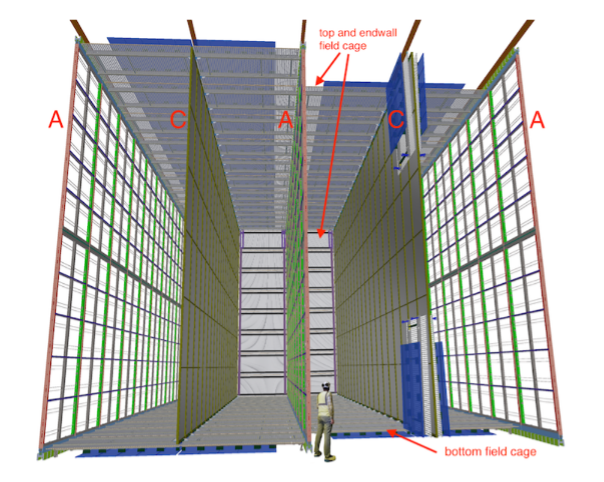
\includegraphics[width=0.7\textwidth]{Hori_Drift.png}
\caption{Distribution of detectors in horizontal drift \cite{Abi_2020}.}
\label{Fig_X1}
\end{figure}


\subsection{DAPHNE and its integration with horizontal drift}

The design and construction of the card for the photon detection system (PDS), which is called DAPHNE (Figure \ref{Fig_X2}), is led by Brazil and some groups from Latin America participate. With cold electronics (CE), both systems are designed to work together to detect and process the photons collected by the SiPMs, which are inside the liquid argon.



\begin{figure}[hbtp]
\centering
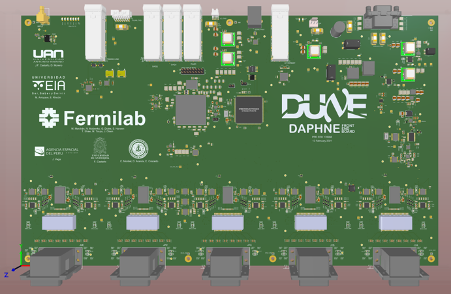
\includegraphics[width=0.7\textwidth]{Daphne.png}
\caption{Design of the DAPHNE acquisition system, each DAPHNE system allows the digitization of 40 independent channels coming from the photon detectors, at a frequency of 62.5 MHz, this information is then transmitted through a Gigabit Ethernet interface.}
\label{Fig_X2}
\end{figure}

DAPHNE's architecture is based on the FELIX system designed at CERN and used for the LHC experiments. The module's PDs will have a lower data rate since the PD electronics, unlike the TPC's, perform zero suppression; therefore, the PDs of a module will be processed. The DAQ will be partitionable: It will be possible to run multiple DAQ instances simultaneously so that most of the detector can take physical data while other DAQ instances run tests for development or special runs, such as calibration runs.

A key philosophy is that all of DUNE's main physical goals can be achieved using only the TPC as a trigger; the information from the PDs can further improve the trigger. There will be two basic triggers in operation. Beam, cosmic, and nucleon decay events will be triggered using the localized high-energy trigger.

Once an activation decision has been made, this will be communicated to the surface and the data will be stored underground until the DAQ BE indicates that it is ready to receive data. The DAQ must also provide the system clock that keeps the detector components in sync and provides the timestamp for all data. To provide finer synchronization between detector components, a 10 MHz reference clock drives the module's 62.5 MHz master clock, which spans all detector components, providing overall synchronization to within 1 ns.



\subsection{Vertical drift as detector array setup}

The vertical drift or dual pass photon detection system is an arrangement of photon detectors that promises to have advantages in the detection of events with respect to the horizontal drift or single pass photon detection, mainly much smaller volumes of liquid Argon could be used, significantly improving the ratio signal-to-noise detection (S/N > 30), is much simpler to build and will allow light to be detected more uniformly at greater distances \cite{Pietropaolo:2792672}.

In this system, the anode and cathode arrangement will be located horizontally, separated by an approximate distance of 6.5 m on the vertical axis, allowing in turn to locate the detection units close to the surface of the Argon and at the base of the cryostat, allowing to stabilize hydrostatic pressure in the container. An electric field of intensity 450 V/cm will be established between the anode and the cathode. For this detector, the displacement of the electrons will be carried out on the vertical axis. Figure \ref{Fig_X3} presents the configuration of the detectors in the setup called vertical drift.


\begin{figure}[hbtp]
\centering
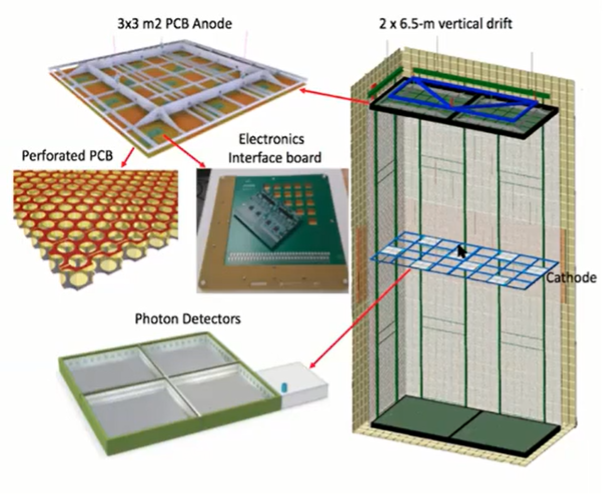
\includegraphics[width=0.7\textwidth]{Vert_Drift.png}
\caption{Distribution of detectors in vertical drift \cite{Abi_2020}.}
\label{Fig_X3}
\end{figure}

\subsection{Problem state}

\subsubsection{Problem to integrate DAPHNE with vertical drift, reduction of its spectrum of applications}

Both horizontal drift and vertical drift are two configurations of photodetectors that have the mission of detecting the interaction between neutrinos and liquid Argon. Despite this, they have two different setups and it is possible that the DAPHNE acquisition system requires different configurations to perform a correct digitization of the stimuli.

These configurations may involve changes to DAPHNE's control software as well as changes to the hardware design, fitting some specific components to improve the detection or new design requirements. Just as it is proposed that the acquisition system can be used with these setups for neutrino detection, new experiments may be considered in the future that require the digitization of high-speed signals for which DAPHNE was designed, but that require of adjustments in its configuration parameters. 

Therefore, it is essential to carry out an analysis and evaluation of the possible modifications that must be made to the DAPHNE board so that it can be used in other experiments or used with different photon detection setups that allow collecting valuable information to answer the questions. raised in the DUNE experiment.




\section{Objectives}
\subsection{General}
\begin{colciencias}
  Enunciado que define de manera concreta el planteamiento del
  problema o necesidad y se inicia con un verbo en modo infinitivo, es
  medible, alcanzable y conlleva a una meta.
\end{colciencias}
\begin{evaluacion}
  Coherencia en la estructura del proyecto:
Articulación y Coherencia entre la pregunta de
investigación, los objetivos, el diseño metodológico y
el cronograma de actividades (que deben incorporar
los componentes y actividades para alcanzar los
objetivos planteados) y los productos esperados. 15
puntos

Concordancia entre el presupuesto total, las
actividades y los objetivos planteados del proyecto.
Justificación adecuada de los rubros, cantidades y
montos solicitados con los objetivos, la metodología
y la duración del proyecto. 5 ptos
\end{evaluacion}
Extract the NSI Wilson coefficients for specific beyond the standard model theories, and check the potential to measure them in present and future neutrino experiments.


To develop and validate software, firmware, and hardware configuration process for the DAPHNE acquisition board for use with one different setup of photodetectors for the detection of photoelectronic stimuli in high-speed applications.
%Desarrollar y validar un proceso de configuración en software, firmware y hardware de la tarjeta de adquisición DAPHNE para su utilización con dos diferentes configuraciones (Setups) de fotodetectores para la detección de estímulos fotoelectrónicos en aplicaciones de alta velocidad.


\subsection{Specifics}
\label{sec:objet-espec}
\begin{colciencias}
  Enunciados que dan cuenta de la secuencia lógica para alcanzar el
  objetivo general del proyecto. No debe confundirse con las
  actividades propuestas para dar alcance a los objetivos (ej. Tomar
  muestras en diferentes localidades de estudio); ni con el alcance de
  los productos esperados (ej. Formar un estudiante de maestría).
\end{colciencias}
\begin{enumerate}
  
\item Study the production of neutrino from pion decays from new mediators 

\item Propose new mechanisms of production of dark matter in intensity
  beams and new experimental techniques for its search supported with
  simulations
  \item Propose new models that produce oscillation effects due to neutrino masses and also NSI interactions
  
\item To evaluate the minimum requirements for the operation of the DAPHNE board and the photodetectors to condition the laboratory following the technical operating conditions of the photodetector configurations in an experimental environment.

\item To design and build one configuration of photodetectors for the detection of photoelectronic stimuli in high-speed applications.

\item To define the necessary configuration in terms of Hardware, Firmware, and Software to couple the DAPHNE acquisition board to the requirements of the photodetector configuration.

\item To validate the performance of the DAPHNE acquisition board in the acquisition of data from high-speed photoelectronic stimuli with a photodetector configuration.


\end{enumerate}


\section{Methodology:                                 }
\begin{colciencias}
  Exposición en forma organizada y precisa de cómo se desarrollará y
  alcanzará el objetivo general y cada uno de los objetivos
  específicos del proyecto, presentando los componentes del mismo y
  las actividades para el logro de estos.
\end{colciencias}
\begin{evaluacion}
  Concordancia entre el presupuesto total, las
actividades y los objetivos planteados del proyecto.
Justificación adecuada de los rubros, cantidades y
montos solicitados con los objetivos, la metodología
y la duración del proyecto.
\end{evaluacion}

Below we present the methodology used to analyze predictions or impose
constraints in models with a dark matter candidate. It is worth
noticing that this methodology has turned into a paradigm after its
use in many models including some of the mentioned before.


\begin{enumerate}

\item The content of particles of the model is selected according to
  the problems to be solved with the criteria defined in the previous
  part of the project.  Once the dark sector is defined, the more
  general Lagrangian is built and all the terms are implemented in a
  the software of high energy physics like SARAH~\cite{Staub:2013tta} or
  FeynRules~\cite{Alloul:2013bka}.
  This will allow us to make the phenomenological analyzes to be
  described in the next steps.  In all the phases, comparisons with
  analytical calculations will be made to be sure of the correctness
  of the obtained results.
  
\item Constraints are imposed from several sources such as neutrino
  physics, lepton flavor violation, direct and indirect DM detection,
  collider searches, etc.

\item For models implemented in SARAH, the Fortran code generated for
  SPheno along with the input files, will be used to build the input
  files for the Fortran/C/C++ code generated for
  micrOMEGAS~\cite{Belanger:2010gh}. This kind of software allows us to
  determine the regions in the parameter space which are consistent
  with the upper limit for the relic density imposed by
  Planck~\cite{Aghanim:2018eyx} and with the upper limits on the
  DM-nucleon cross-section imposed by the direct detection experiments
  like LUX~\cite{Akerib:2018lyp}, PandaX-II~\cite{Tan:2016diz} and
  XENON1T~\cite{Aprile:2017iyp}.
  We will also obtain the region of the parameter space to be explored
  by future direct detection experiments like LZ~\cite{Akerib:2018lyp}
  and DARWIN~\cite{Aalbers:2016jon}.
  In addition, we will check for the impact of indirect detection dark
  matter experiments, present and future, like
  Fermi-LAT~\cite{Ajello:2018sxm}, HESS~\cite{Abdallah:2016ygi},
  IceCube~\cite{Iovine:2019rmd}, AMS-02~\cite{Giovacchini:2020vxz},
  CTA~\cite{Acharya:2017ttl}, DAMPE~\cite{Jiang:2020jbc}.
  For this project is is specially relevant take in consideration the constraints in the kinetic mixing between
  the dark photon and the photon obtained from direct detection experiments
  like PandaX-II \cite{Ren:2018gyx}, and CDEX-10~\cite{She:2019skm}.
  

  In the case for which the WIMP turn out to be subdominant component
  of the early Universe plasma, we further extend the model with
  either new dark matter particles or non-standard cosmology.

\item In the models with DM candidates which are singlets under the standard
  model, we will further consider SIMP or FIMP mechanisms to produce
  the proper relic density in order to open new regions of the
  parameter space compatible with direct and indirect dark matter
  searches. In this case owned codes will be used.

\item With the generated Python code for
  MadGraph~\cite{Alwall:2011uj}, along with the required input files
  from SPheno, we will make simulations of the signal in several
  particle detectors, including the ones for DUNE. For this purpose,
  samples of MadGraph events are used with hadronization through
  Pythia~\cite{Sjostrand:2014zea} and with some extra software component for the
  simulation of the detector, like Delphes~\cite{deFavereau:2013fsa} for the case of the
  LHC.
  If the signal have been already implemented by the experimental
  collaborations and the results are available, we can use computation
  codes like CheckMATE~\cite{Drees:2013wra} to recast the results for
  our specific model.

  If the signal is not already implemented by the LHC experimental
  collaborations or in CheckMATE~\cite{Drees:2013wra}, we will further
  require to implement the background generation and design the best
  set of cuts to establish the significance to measurement the signal
  upon the background in a such a way that the regions of discovery
  can be established.


\end{enumerate}

For each Lagrangian implemented in SARAH with the input/output codes
for SPheno, MicrOMEGAS, and MadGraph, then, the software and produced
data will follow a reproducibility protocol of scientific result by
following the methodology explained in the paper entitled: ``Ten
simple rules for writing and sharing computational analyses in Jupyter
Notebooks''~\cite{Rule2019}.  There is included the necessary
mechanisms to have the used methodology correctly referenced inside
the resulting scientific paper. In particular, the way in which the
created software must be organized as open source \url{https://GitHub.com} repositories.
All the resulting preprints will be submitted to the arXiv.org repository along with the submission to
the top journals in our area. All of them  are now Open Access without cost for the authors through the
SCOAP3 consortium \url{https://scoap3.org}. 
Therefore  the project  will follow all the high 
standards of the Open Science methodology.

Every step in the methodology requires the intensive use of computational tools.
The project has already the supercomputer clusters  in each of
the participant institutions.

It is worth noticing that the one in the Universidad de Antioquia, now for
use of the full institution,
is currently maintained by the research Group
participating in this project.  Therefore, all the improvements in
hardware and software associated with this project, immediately have
an impact in all users of the system, especially for the people working
with big data and data mining.  In particular, the ColaV group for
scientometric analysis at Universidad de Antioquia
\url{https://colav.github.io} have been directly benefited from the
Jupyter notebook service for big data analysis implemented for this
kind of projects.


\subsection{Experimental methodology}

In the experimental part, this project focuses on validating and configuring the design of the DAPHNE board for its application in different detection experiments that require the acquisition of high-speed photoelectronic stimuli. In this way, the proposed methodology will address three components, in the first instance the technological update regarding the implementation of a photoelectron detection setup, in the second instance the design and construction of different photodetector setups and their coupling with the acquisition board DAPHNE, and in the third instance the validation of the modifications in the DAPHNE board and the standardization of the configuration for the coupling of the different setups with DAPHNE. Accordingly, the main activities to be carried out are the following:

\begin{enumerate}
    \item Constant updating in the state of the art about the implementation of photodetector setups for the detection of photoelectronic stimuli, a constant search will be made for the latest advances in the design and construction of experiments based on the photodetection of this type of phenomenon, mainly aligned in the detection requirements provided by the DUNE collaboration, but without limiting the application of the acquisition system to this single application environment.
    
    \item Evaluation of a setup previously tested with DAPHNE and replicate the conditions of the experiment to obtain similar results. Currently the DUNE collaboration is running a proto-DUNE experiment, in this experiment performance tests are being carried out on a photodetection setup called "Far Detector Single-phase" as well as the performance of the acquisition board DAPHNE \cite{Abi_2020}. According to this, it is necessary to build a photodetector setup previously tested with DAPHNE and replicate the conditions of the experiment, since to validate the configuration for different photodetector setups it is first necessary to have reference measurements in the laboratory comparable with those obtained in the real environment of the experiment.
    
    \item Design and build a photodetector setup based on requirements for the detection of photoelectrons in experiments similar to those being carried out in the DUNE collaboration and in particular in the proto-DUNE experiment. For this it is necessary to evaluate the technical requirements of the setups previously built for the proto-DUNE experiment. This evaluation of requirements is carried out from the electronic design, mechanical design, selection of high performance components, cryogenic tests or in environments emulating similar conditions of the experiment, among others.
    
    \item Perform high-speed data acquisition tests using the DAPHNE board and the new setup. Carrying out the technical evaluation of the conditions of the experiment and checking the operation of the DAPHNE board against different configurations in hardware, firmware and software.
    
    \item Identify and implement changes in the hardware, firmware and software configuration of the DAPHNE board based on the measurements made with the built setup. It is necessary to evaluate the capacity of the DAPHNE board to adapt to different conditions and experimental setups in the detection of photoelectronic stimuli. Through this identification it is proposed to execute modifications in the design of the DAPHNE board that allow it to obtain high performance measurements in different applications and that allow it to work in optimal conditions with different setups.
    
    \item Carry out a comparative analysis of the performance of the Daphne card by analyzing the data obtained for a reference setup and a new setup for photoelectronic stimulus detection experiments. This will allow standardizing the appropriate configuration for the DAPHNE board, verifying that the performance is similar when the setup is tested with two different DAPHNE boards.
    
    
\end{enumerate}



\section{Candidate's contribuition} 


  Orlando L.G. Peres has experience in neutrino phenomenology and it
  will contribute to connecting the models proposed to the existent
  constraints on neutrino physics. For a given model, these can
  non-standard neutrino interaction effects (NSI), neutrino decay
  effects and many other consequences that it can be tested more
  deeply using a combined analysis of neutrino experiments.
  
  The Colombian counterpart of the researcher's team has a great experience 
  proposing and studying renormalizable dark matter models that account
  for the massiveness of active neutrinos. For instance, the work presented in \cite{Restrepo:2013aga} contains a list of 35 models at the TeV-scale
  that are compatible with neutrino masses and dark matter. More recently, 
  a similar analysis for Dirac neutrinos was made, by finding the five minimal models
  which develop the one-loop topologies with a single gauge Abelian symmetry which explains both the smallness of neutrino masses and the stability of the dark matter
  candidate~\cite{Calle:2018ovc}. It is complemented with the newfound model of
  one-loop Dirac neutrino masses with Majorana neutrinos, which constitutes the first example of a non-trivial pure Dark symmetry in which the Dark photon is a mediator from dark matter to neutrino physics~\cite{Calle:2019mxn}.
  For the usual $\operatorname{U}(1)_{B-L}$-symmetry in which the extra gauge 
  mediator have been heavily constrained from the LHC searches~\cite{Chiang:2019ajm},
  a more systematic study with the possibilities at one and two-loops for Dirac neutrino masses have accomplished in~\cite{Jana:2019mgj}.
  %
  Furthermore, the possible connection between neutrino masses and other 
  dark matter candidates as the axion has been explored~\cite{Carvajal:2018ohk}.  
  In addition to the project's tasks concerning phenomenological 
  analysis of dark matter, Oscar Zapata will be also in charge of identifying 
  relevant new terms as sources of non-standard neutrino interactions,  and exploring scenarios that require
  dark matter production mechanisms beyond the WIMP paradigm or a 
  non-standard cosmology 
  (scenarios having several dark matter candidates may be also considered).
  %
  On the other hand, Diego Restrepo features a large experience on
  phenomenological analysis of models beyond the standard model, in
  particular, with high-performance simulations for particle collider
  and detectors. Additionally, José David Ruiz-Álvarez has experience
  in the study and simulation of events from collider as a
  phenomenologist and as a CMS experiment researcher. This will allow
  the assessment of the production and detection of dark photons in
  the DUNE experiment from a phenomenological approach for the models
  developed in this research program.  William Ponce, now an Emeritus
  professor at Universidad de Antioquia, is a leading expert in 331
  models, and now is working in Abelian gauge extensions. In this
  project he will search for the possibility of having dark photons
  within 331 SM extensions.
  
  
  \subsection{Added value to be expected from the collaboration}
  Within a large portion of scotogenic models (dark matter models with 
  radiative neutrino masses) it is possible to build non renormalizable
  operators that induce non-standard neutrino interactions which may lead
  to novel signatures to be detected at current and future neutrino experiments. 
  This constitutes one of the samples where the collaboration between the two sides
  would enhance the research results of the project. 
  
  
  The trajectory of the colombian team with simulations for production
  and detection of new particles in collider along with the
  accumulated knowledge about the DUNE experiment by the brazilian
  team will facilitate the proposal of new production and detection
  techniques of dark photons in the DUNE experiment.
%  \section{Timeline}
%  {\it A clear description of the planned collaboration (distribution of work per year/per side and methods of implementation) and the added value to be expected from the collaboration.}
  
\section{Foreseen actions and expected results}
Two seminars by the Colombian researchers during their visits to Brazil will take place. Moreover,  at the end of the project the Colombian counterpart will present a seminar along with a dissemination talk at University of Antioquia.  

We propose to made {\it Hack Days}, a brainstorm of the experience researchers and the graduate students into a {\it one-week} workshop to be happening once in Brazil and in Colombia.

\subsection{New-Knowledge Products}


By the end of the project we expect at least 3 joint publications (A1 or A2) regarding new scotogenic models and their dark matter phenomenology,  discovery potential at the LHC and future collider of massive neutrinos and/or dark matter models, and sensitivity of future neutrino experiments to non-standard neutrino interactions.

\subsection{ Social-Appropriation-of-Knowledge Products}

A product of social-appropriation-of-knowledge about generation of outreach content:  multimedia product about research results.
The researchers of this project will participate in the organization of an scientific event in Colombia, in particular in the already successful yearly series of ``Colombian Meeting of High Energy Physics'' (ComHEP) or ``Materia Oscura Colombia'' (MOCA).

\subsection{Human-Resource Training}
One master student and participation of other master student.
\section{Plans for future collaborations}
We consider this first collaborative project between the high energy physics group of the University of Antioquia with Profs. Peres and Segreto as the beginning of a long and fruitful scientific collaboration due to the symbiotic and common strengths. 
Therefore we expect such a collaboration to continue beyond the end of this grant, for instance through the submission of research proposal to Colciencias grants from the colombian counterpart, mobility of MSc and PhD students and researchers from both countries, etc.      


%%% Local Variables: 
%%% mode: latex
%%% TeX-master: "proyecto"
%%% ispell-local-dictionary: "american"
%%% End: 



\section{Budget in Colombian Pesos}
\begin{itemize}
    \item Travels: 50 million
    \item Master Student: 50 millions
    \item Equipment's: 50 millions
\end{itemize}
TOTAL=150 millions



% Style can be changed if desired
%\bibliographystyle{vitae}
\bibliographystyle{jhep}
\bibliography{refs}


\end{document}

	  
